\question[20] Two insulating spherical shells with different radii share a common center. The inner shell has a radius $R_1=5$ cm and carries a charge of $-25$ nC distributed uniformly around its surface. The outer shell has a radius $R_2=8$ cm and carries a charge of $+64$ nC distributed uniformly around its surface. 


\begin{center}
	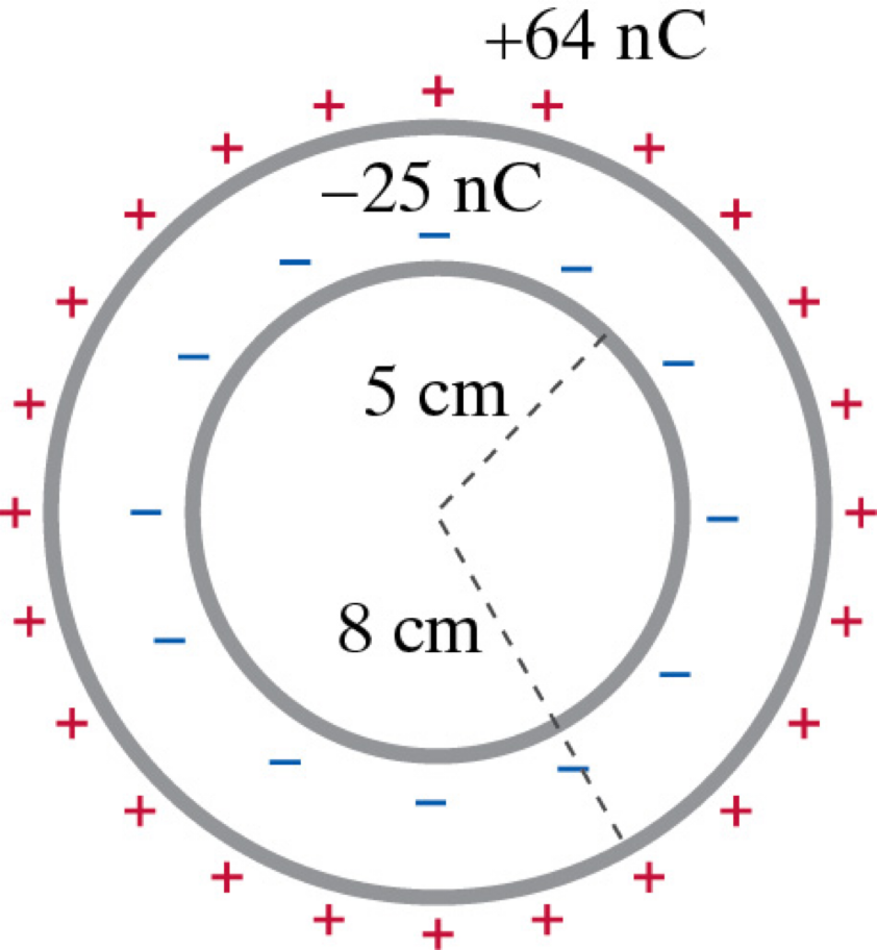
\includegraphics[width=.4\textwidth]{concentric_shells.pdf}
\end{center}


You measure the magnetic field at point $A$ and find that it is zero at that location.
\begin{parts}
	\part What is the electric field (both magnitude and direction) at a distance of $3$ cm away from the center?
	\vspace{3cm}
	\part What is the electric field (both magnitude and direction) at a distance of $7$ cm away from the center?	
	\vspace{3cm}
	\part What is the electric field (both magnitude and direction) at a distance of $10$ cm away from the center?		
\end{parts}